\documentclass[11pt,a4paper]{report}
\usepackage[textwidth=37em,vmargin=30mm]{geometry}
\usepackage{calc,xunicode,amsmath,amssymb,paralist,enumitem,tabu,booktabs,datetime2,xeCJK,xeCJKfntef,listings}
\usepackage{tocloft,fancyhdr,tcolorbox,xcolor,graphicx,eso-pic,xltxtra,xelatexemoji}

\newcommand{\envyear}[0]{2025}
\newcommand{\envdatestr}[0]{2025-09-20}
\newcommand{\envfinaldir}[0]{webdb/2025/20250920/final}

\usepackage[hidelinks]{hyperref}
\hypersetup{
    colorlinks=false,
    pdfpagemode=FullScreen,
    pdftitle={Web Digest - \envdatestr}
}

\setlength{\cftbeforechapskip}{10pt}
\renewcommand{\cftchapfont}{\rmfamily\bfseries\large\raggedright}
\setlength{\cftbeforesecskip}{2pt}
\renewcommand{\cftsecfont}{\sffamily\small\raggedright}

\setdefaultleftmargin{2em}{2em}{1em}{1em}{1em}{1em}

\usepackage{xeCJK,xeCJKfntef}
\xeCJKsetup{PunctStyle=plain,RubberPunctSkip=false,CJKglue=\strut\hskip 0pt plus 0.1em minus 0.05em,CJKecglue=\strut\hskip 0.22em plus 0.2em}
\XeTeXlinebreaklocale "zh"
\XeTeXlinebreakskip = 0pt


\setmainfont{Brygada 1918}
\setromanfont{Brygada 1918}
\setsansfont{IBM Plex Sans}
\setmonofont{JetBrains Mono NL}
\setCJKmainfont{Noto Serif CJK SC}
\setCJKromanfont{Noto Serif CJK SC}
\setCJKsansfont{Noto Sans CJK SC}
\setCJKmonofont{Noto Sans CJK SC}

\setlength{\parindent}{0pt}
\setlength{\parskip}{8pt}
\linespread{1.15}

\lstset{
	basicstyle=\ttfamily\footnotesize,
	numbersep=5pt,
	backgroundcolor=\color{black!5},
	showspaces=false,
	showstringspaces=false,
	showtabs=false,
	tabsize=2,
	captionpos=b,
	breaklines=true,
	breakatwhitespace=true,
	breakautoindent=true,
	linewidth=\textwidth
}






\newcommand{\coverpic}[2]{
    % argv: itemurl, authorname
    Cover photo by #2~~(\href{#1}{#1})
}
\newcommand{\makeheader}[0]{
    \begin{titlepage}
        % \newgeometry{hmargin=15mm,tmargin=21mm,bmargin=12mm}
        \begin{center}
            
            \rmfamily\scshape
            \fontspec{BaskervilleF}
            \fontspec{Old Standard}
            \fontsize{59pt}{70pt}\selectfont
            WEB\hfill DIGEST
            
            \vfill
            % \vskip 30pt
            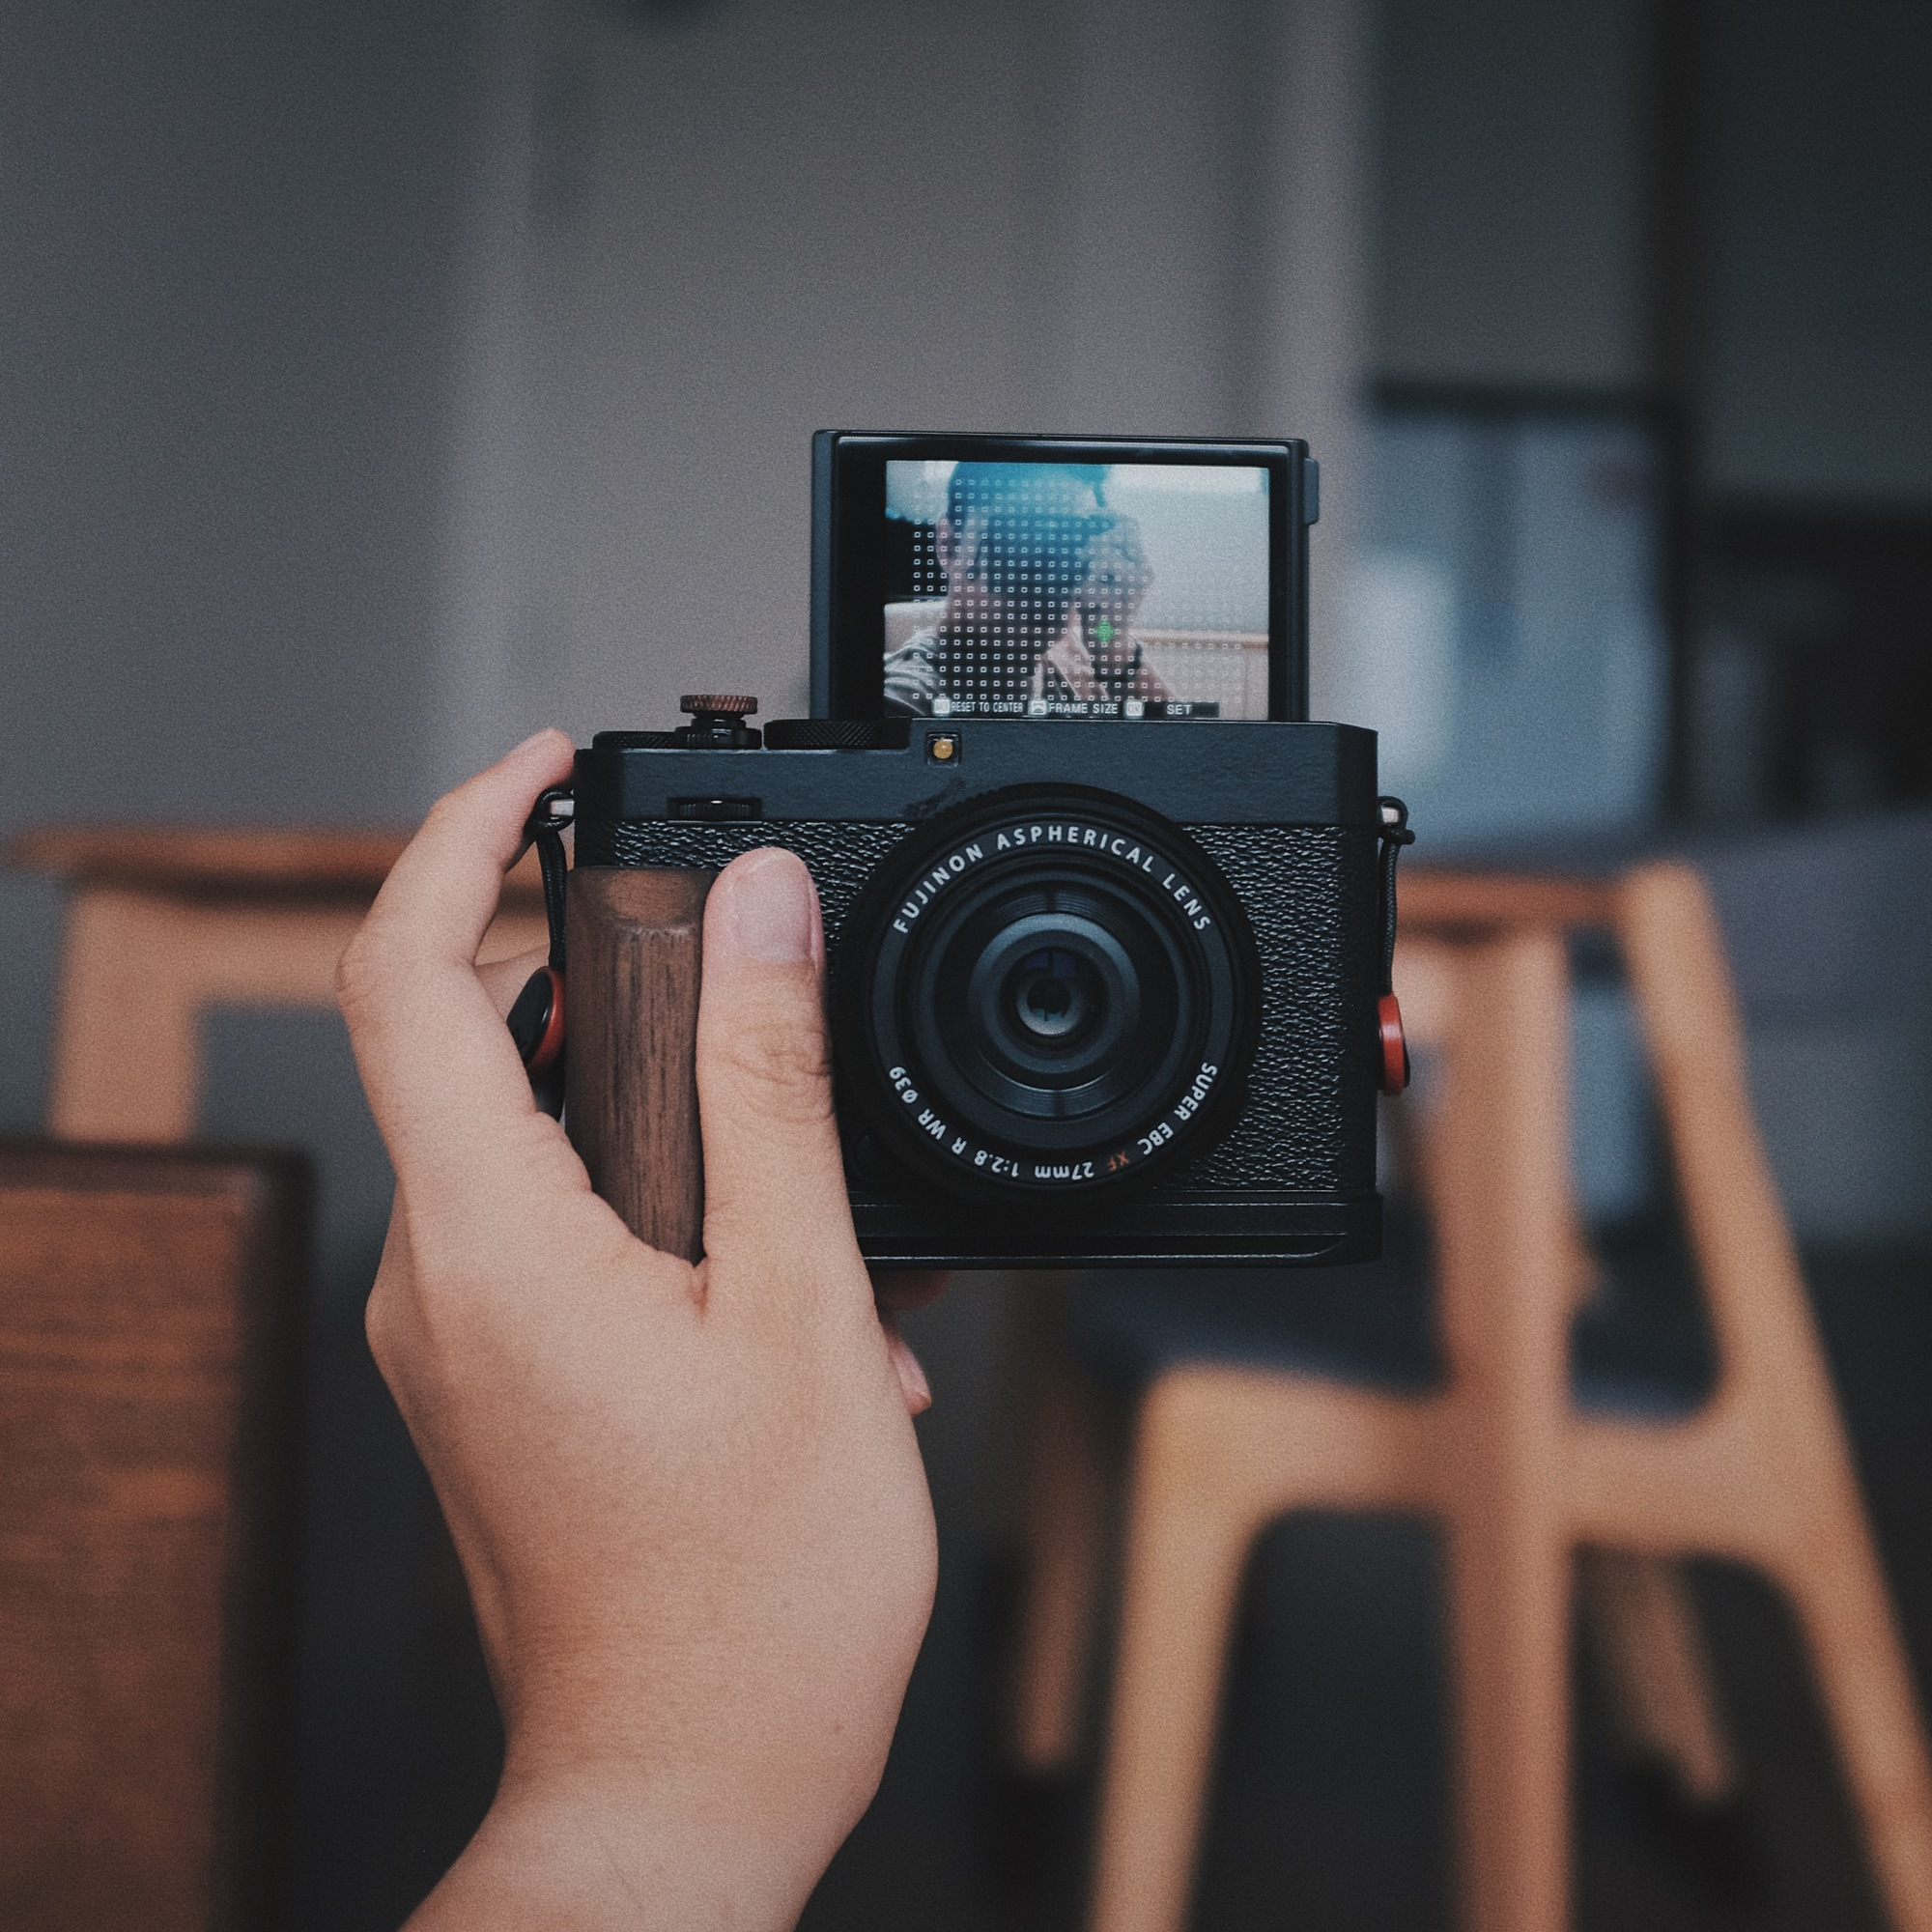
\includegraphics[width=\linewidth]{\envfinaldir/coverpic-prod.jpg}\par
            % \vskip 30pt
            \vfill

            \normalsize\rmfamily\scshape
            \copyright{} The Web Digest Project \hfill\large \envdatestr
        \end{center}
    \end{titlepage}
    % \restoregeometry
}
\newcommand{\simplehref}[1]{%
    \textcolor{blue!80!green}{\href{#1}{#1}}%
}
\renewcommand{\contentsname}{\center\Huge\sffamily\bfseries Contents\par\vskip 20pt}
\newcounter{ipartcounter}
\setcounter{ipartcounter}{0}
\newcommand{\ipart}[1]{
    % \vskip 20pt
    \clearpage
    \stepcounter{ipartcounter}
    \phantomsection
    \addcontentsline{toc}{chapter}{#1}
    % \begin{center}
    %     \Huge
    %     \sffamily\bfseries
    %     #1
    % \end{center}
    % \vskip 20pt plus 7pt
}
\newcounter{ichaptercounter}
\setcounter{ichaptercounter}{0}
\newcommand{\ichapter}[1]{
    % \vskip 20pt
    \clearpage
    \stepcounter{ichaptercounter}
    \phantomsection
    \addcontentsline{toc}{section}{\numberline{\arabic{ichaptercounter}}#1}
    \begin{center}
        \Huge
        \sffamily\bfseries
        #1
    \end{center}
    \vskip 20pt plus 7pt
}
\newcommand{\entrytitlefont}[1]{\subsection*{\raggedright\Large\sffamily\bfseries#1}}
\newcommand{\entryitemGeneric}[2]{
    % argv: title, url
    \parbox{\linewidth}{
        \entrytitlefont{#1}\par\vskip 5pt
        \footnotesize\ttfamily\mdseries
        \simplehref{#2}
    }\vskip 11pt plus 11pt minus 1pt
}
\newcommand{\entryitemGithub}[3]{
    % argv: title, url, desc
    \parbox{\linewidth}{
        \entrytitlefont{#1}\par\vskip 5pt
        \footnotesize\ttfamily\mdseries
        \simplehref{#2}\par\vskip 5pt
        \small\rmfamily\mdseries#3
    }\vskip 11pt plus 11pt minus 1pt
}
\newcommand{\entryitemAp}[3]{
    % argv: title, url, desc
    \parbox{\linewidth}{
        \entrytitlefont{#1}\par\vskip 5pt
        \footnotesize\ttfamily\mdseries
        \simplehref{#2}\par\vskip 5pt
        \small\rmfamily\mdseries#3
    }\vskip 11pt plus 11pt minus 1pt
}
\newcommand{\entryitemHackernews}[3]{
    % argv: title, hnurl, rawurl
    % \parbox{\linewidth}{
    %     \entrytitlefont{#1}\par\vskip 5pt
    %     \footnotesize\ttfamily\mdseries
    %     \simplehref{#3}\par
    %     \textcolor{black!50}{\href{#2}{#2}}
    % }\vskip 11pt plus 11pt minus 1pt
    \begin{minipage}{\linewidth}
            \entrytitlefont{#1}\par\vskip 5pt
            \footnotesize\ttfamily\mdseries
            \simplehref{#3}\par
            \textcolor{black!50}{\href{#2}{#2}}
    \end{minipage}\par\vskip 11pt plus 11pt minus 1pt
}







\begin{document}

\makeheader

\tableofcontents\clearpage




\ipart{Developers}
\ichapter{Hacker News}
\entryitemTwoLinks{Ask HN: Has anyone else been unemployed for over two years?}{https://news.ycombinator.com/item?id=45306539}{https://news.ycombinator.com/item?id=45306539}

\entryitemTwoLinks{Trump to impose \$100k fee for H-1B worker visas, White House says}{https://news.ycombinator.com/item?id=45305845}{https://www.reuters.com/business/media-telecom/trump-mulls-adding-new-100000-fee-h-1b-visas-bloomberg-news-reports-2025-09-19/}

\entryitemTwoLinks{Internal emails reveal Ticketmaster helped scalpers jack up prices, FTC says}{https://news.ycombinator.com/item?id=45305042}{https://arstechnica.com/tech-policy/2025/09/ticketmaster-intentionally-screwed-fans-out-of-billions-ftc-lawsuit-says/}

\entryitemTwoLinks{After getting Jimmy Kimmel suspended, FCC chair threatens ABC's The View}{https://news.ycombinator.com/item?id=45304992}{https://arstechnica.com/tech-policy/2025/09/after-getting-jimmy-kimmel-suspended-fcc-chair-threatens-abcs-the-view/}

\entryitemTwoLinks{A shift in developer culture is impacting innovation and creativity}{https://news.ycombinator.com/item?id=45303199}{https://dayvster.com/blog/dev-culture-is-dying-the-curious-developer-is-gone/}

\entryitemTwoLinks{Trevor Milton's Nikola case dropped by SEC following Trump pardon}{https://news.ycombinator.com/item?id=45302220}{https://eletric-vehicles.com/nikola/trevor-miltons-nikola-case-dropped-by-sec-following-trump-pardon/}

\entryitemTwoLinks{I regret building this \$3000 Pi AI cluster}{https://news.ycombinator.com/item?id=45302065}{https://www.jeffgeerling.com/blog/2025/i-regret-building-3000-pi-ai-cluster}

\entryitemTwoLinks{As Android developer verification gets ready to go, a new reason to be worried}{https://news.ycombinator.com/item?id=45301845}{https://www.androidauthority.com/android-sideload-offline-3598988/}

\entryitemTwoLinks{Intel Arc Celestial dGPU seems to be first casualty of Nvidia partnership}{https://news.ycombinator.com/item?id=45301679}{https://www.notebookcheck.net/Intel-Arc-Celestial-dGPU-seems-to-be-first-casualty-of-Nvidia-partnership-while-Intel-Arc-B770-is-allegedly-still-alive.1118962.0.html}

\entryitemTwoLinks{Ask HN: Does anyone else notice YouTube causing 100\% CPU usage and stattering?}{https://news.ycombinator.com/item?id=45301499}{https://news.ycombinator.com/item?id=45301499}

\entryitemTwoLinks{The sordid reality of retirement villages: Residents are being milked for profit}{https://news.ycombinator.com/item?id=45301403}{https://unherd.com/2025/09/the-sordid-truth-about-retriement-villages/}

\entryitemTwoLinks{Ants that seem to defy biology – They lay eggs that hatch into another species}{https://news.ycombinator.com/item?id=45300865}{https://www.smithsonianmag.com/smart-news/these-ant-queens-seem-to-defy-biology-they-lay-eggs-that-hatch-into-another-species-180987292/}

\entryitemTwoLinks{YouTube downloaders (and how Google silenced the press)}{https://news.ycombinator.com/item?id=45300810}{https://windowsread.me/p/best-youtube-downloaders}

\entryitemTwoLinks{Statistical Physics with R: Ising Model with Monte Carlo}{https://news.ycombinator.com/item?id=45299625}{https://github.com/msuzen/isingLenzMC}

\entryitemTwoLinks{Ruby Central's Attack on RubyGems [pdf]}{https://news.ycombinator.com/item?id=45299170}{https://pup-e.com/goodbye-rubygems.pdf}

\entryitemTwoLinks{iTerm2 Web Browser}{https://news.ycombinator.com/item?id=45298793}{https://iterm2.com/documentation-web.html}

\entryitemTwoLinks{Nostr}{https://news.ycombinator.com/item?id=45298336}{https://nostr.com/}

\entryitemTwoLinks{The health benefits of sunlight may outweigh the risk of skin cancer}{https://news.ycombinator.com/item?id=45298034}{https://www.economist.com/science-and-technology/2025/09/17/the-health-benefits-of-sunlight-may-outweigh-the-risk-of-skin-cancer}

\entryitemTwoLinks{Gemini in Chrome}{https://news.ycombinator.com/item?id=45297331}{https://gemini.google/overview/gemini-in-chrome/}

\entryitemTwoLinks{Playing ``Minecraft'' without Minecraft (2024)}{https://news.ycombinator.com/item?id=45297258}{https://lenowo.org/viewtopic.php?t=5}\ichapter{Phoronix}
\entryitemGeneric{\hskip 0pt{}Linux 6.17 File-System Benchmarks, Including OpenZFS \& Bcachefs}{https://www.phoronix.com/review/linux-617-filesystems}

\entryitemGeneric{\hskip 0pt{}Mesa Adds Contributor Guidelines - Will Allow AI Generated Code If Author Understands It}{https://www.phoronix.com/news/Mesa-Contributor-Guidelines}

\entryitemGeneric{\hskip 0pt{}Ubuntu Now Has Daily Dangerous Desktop Images}{https://www.phoronix.com/news/Ubuntu-Daily-Dangerous}

\entryitemGeneric{\hskip 0pt{}Zink OpenGL-On-Vulkan Driver Tackles OpenGL Mesh Shaders}{https://www.phoronix.com/news/Zink-Mesh-Shaders-Ready}

\entryitemGeneric{\hskip 0pt{}AMDKFD Compute Driver Sees Patches For S0ix Standby Support}{https://www.phoronix.com/news/AMDKFD-Compute-S0ix}

\entryitemGeneric{\hskip 0pt{}KDE Plasma 6.5 Beta Released With KNightTime, Rounded Bottom Window Corners}{https://www.phoronix.com/news/KDE-Plasma-6.5-Beta-Released}

\entryitemGeneric{\hskip 0pt{}Ubuntu 25.10 Beta Officially Released For Testing}{https://www.phoronix.com/news/Ubuntu-25.10-Beta}

\entryitemGeneric{\hskip 0pt{}Steam Will End Windows 32-bit OS Support Next Year - Hopefully Linux Follows}{https://www.phoronix.com/news/Steam-Ending-32-bit-Windows}

\entryitemGeneric{\hskip 0pt{}PCIe 8.0 v0.3 Specification Released To Members}{https://www.phoronix.com/news/PCI-Express-8.0-v0.3}


\ipart{Developers~~~~(zh-Hans)}
\ichapter{Solidot}
\entryitemGeneric{\hskip 0pt{}汽车行业制造了远超需求的汽车}{https://www.solidot.org/story?sid=82363}

\entryitemGeneric{\hskip 0pt{}Steam 将从 2026 年起不再支持 32 位 Windows 操作系统}{https://www.solidot.org/story?sid=82362}

\entryitemGeneric{\hskip 0pt{}新材料拉伸率达到 46 倍且能自我修复}{https://www.solidot.org/story?sid=82361}

\entryitemGeneric{\hskip 0pt{}2025 年度搞笑诺贝尔奖宣布}{https://www.solidot.org/story?sid=82360}

\entryitemGeneric{\hskip 0pt{}Google 为美国用户的 Chrome 浏览器集成 Gemini AI 功能}{https://www.solidot.org/story?sid=82359}

\entryitemGeneric{\hskip 0pt{}三星推送软件更新为冰箱加入广告}{https://www.solidot.org/story?sid=82358}

\entryitemGeneric{\hskip 0pt{}斑胸草雀具有语义理解能力}{https://www.solidot.org/story?sid=82357}

\entryitemGeneric{\hskip 0pt{}英伟达向英特尔投资 50 亿美元}{https://www.solidot.org/story?sid=82356}

\entryitemGeneric{\hskip 0pt{}研究发现珊瑚无法在一个更温暖的世界里生存下来}{https://www.solidot.org/story?sid=82355}

\entryitemGeneric{\hskip 0pt{}DeepSeek 发表 R1 模型论文,称训练成本仅 29.4 万美元}{https://www.solidot.org/story?sid=82354}

\entryitemGeneric{\hskip 0pt{}全球变暖致日本危险性高温日增加 22 天}{https://www.solidot.org/story?sid=82353}

\entryitemGeneric{\hskip 0pt{}NASA 确认了逾六千颗系外行星}{https://www.solidot.org/story?sid=82352}

\entryitemGeneric{\hskip 0pt{}最黑暗的夜晚愈来愈亮}{https://www.solidot.org/story?sid=82351}

\entryitemGeneric{\hskip 0pt{}电视的黄金时代可能已经结束}{https://www.solidot.org/story?sid=82350}

\entryitemGeneric{\hskip 0pt{}极端高温催生新法律保护工人}{https://www.solidot.org/story?sid=82349}

\entryitemGeneric{\hskip 0pt{}美国国会要求 Valve、Discord 和 Twitch CEO 就用户激进化作证}{https://www.solidot.org/story?sid=82348}

\entryitemGeneric{\hskip 0pt{}小鹏汇天两辆飞行汽车在长春航展上相撞}{https://www.solidot.org/story?sid=82347}

\entryitemGeneric{\hskip 0pt{}GNOME 49 释出}{https://www.solidot.org/story?sid=82346}

\entryitemGeneric{\hskip 0pt{}黑猩猩每天食用熟果摄入的酒精量相当于一瓶啤酒}{https://www.solidot.org/story?sid=82345}

\entryitemGeneric{\hskip 0pt{}ChatGPT 将估计用户年龄,可能要求验证年龄}{https://www.solidot.org/story?sid=82344}\ichapter{V2EX}
\entryitemGeneric{\hskip 0pt{}[酷工作] 资深全栈开发/后端 [可远程]}{https://www.v2ex.com/t/1160643}

\entryitemGeneric{\hskip 0pt{}[问与答] 深圳有没有靠谱的 iPhone 换电池商家?想当场换}{https://www.v2ex.com/t/1160642}

\entryitemGeneric{\hskip 0pt{}[投资] 是时候减仓纳指 100 了}{https://www.v2ex.com/t/1160640}

\entryitemGeneric{\hskip 0pt{}[问与答] 绑定邮箱不支持 foxmail?}{https://www.v2ex.com/t/1160639}

\entryitemGeneric{\hskip 0pt{}[买买买] 话说有没有老 thinkpad 推荐?}{https://www.v2ex.com/t/1160638}

\entryitemGeneric{\hskip 0pt{}[分享创造] [自荐] Lucy Edit AI | 一个免费的 AI 视频编辑网站}{https://www.v2ex.com/t/1160637}

\entryitemGeneric{\hskip 0pt{}[推广] Luma Ray3:真的能碾压 VEO3 和 Runway 吗?}{https://www.v2ex.com/t/1160636}

\entryitemGeneric{\hskip 0pt{}[程序员] XXL-TOOL v2.1.0 发布 | Java 工具类库}{https://www.v2ex.com/t/1160635}

\entryitemGeneric{\hskip 0pt{}[计算机] 有无 Ray3 API 供应商}{https://www.v2ex.com/t/1160634}

\entryitemGeneric{\hskip 0pt{}[酷工作] ETL 数据工程师,远程办公, 3-4 个月短期项目}{https://www.v2ex.com/t/1160632}

\entryitemGeneric{\hskip 0pt{}[问与答] 大家有觉得小米红米的电子产品寿命不行么}{https://www.v2ex.com/t/1160631}

\entryitemGeneric{\hskip 0pt{}[Windows] 才装了一个星期的 Windows 电脑,「系统与保留」占据了 74.3GB 正常吗?}{https://www.v2ex.com/t/1160630}

\entryitemGeneric{\hskip 0pt{}[奇思妙想] 零食店的收银机竟然是视频识别}{https://www.v2ex.com/t/1160629}

\entryitemGeneric{\hskip 0pt{}[问与答] 2025 年最便宜的 s3 有哪些值得推荐?}{https://www.v2ex.com/t/1160627}

\entryitemGeneric{\hskip 0pt{}[Windows] Windows 台式机外接显示屏上总是时不时出现闪动的短横线亮斑}{https://www.v2ex.com/t/1160625}

\entryitemGeneric{\hskip 0pt{}[问与答] 求推荐静音的家里用的机架式服务器}{https://www.v2ex.com/t/1160624}

\entryitemGeneric{\hskip 0pt{}[Go 编程语言] 2025 (非预制) Vue 3 + Golang 全栈课 - 第一讲}{https://www.v2ex.com/t/1160623}

\entryitemGeneric{\hskip 0pt{}[分享发现] 是不是最近 pcdn 少了,我发现抖音刷起来每次 n 次卡主 需要往后拉或者上下刷}{https://www.v2ex.com/t/1160621}

\entryitemGeneric{\hskip 0pt{}[职场话题] 靠,北京市政府终于公布了 2025 年社保缴费基数了,果然三险+医疗保险又尼玛涨了!}{https://www.v2ex.com/t/1160620}

\entryitemGeneric{\hskip 0pt{}[分享发现] 我发现 Astro Wind 写的产品官网挺好看的,加上用 AI 辅助生成内容,一个小时就写好了还挺美观的}{https://www.v2ex.com/t/1160618}

\entryitemGeneric{\hskip 0pt{}[汽车] ix3 还是 ES6}{https://www.v2ex.com/t/1160617}

\entryitemGeneric{\hskip 0pt{}[宽带症候群] 国庆出游到新疆,只带了手机,建议访问 v2 吗?}{https://www.v2ex.com/t/1160616}

\entryitemGeneric{\hskip 0pt{}[分享创造] 教零代码 / AI 基础的媳妇 2 小时做出了动物图片转 MP4 工具,分享给大家!}{https://www.v2ex.com/t/1160613}

\entryitemGeneric{\hskip 0pt{}[MacBook] 咸鱼 m3 max 128G 8T,卖 26000 正常吗?}{https://www.v2ex.com/t/1160610}

\entryitemGeneric{\hskip 0pt{}[问与答] 有没有良方可以治穷病}{https://www.v2ex.com/t/1160609}

\entryitemGeneric{\hskip 0pt{}[Apple] 全家手机马上要换成 iPhone 了,怎么配置 iCloud 和 apple music 的家庭套餐最便宜?}{https://www.v2ex.com/t/1160608}

\entryitemGeneric{\hskip 0pt{}[职场话题] 29 岁, 7 年前端转型 AI,在合肥遇到一个纠结的 Offer,该不该接?}{https://www.v2ex.com/t/1160607}

\entryitemGeneric{\hskip 0pt{}[投资] [求合作] 你有流量我有资源,合作共赢!}{https://www.v2ex.com/t/1160606}

\entryitemGeneric{\hskip 0pt{}[macOS] macbook 系统数据很大问题咨询}{https://www.v2ex.com/t/1160605}

\entryitemGeneric{\hskip 0pt{}[Apple] macOS 26 的重大更新其实是引入了「手记」mac 版}{https://www.v2ex.com/t/1160604}

\entryitemGeneric{\hskip 0pt{}[问与答] 某手机厂商 在 新机发布时 会对旧手机的性能 云控限制 , 这是真的吗?}{https://www.v2ex.com/t/1160602}

\entryitemGeneric{\hskip 0pt{}[生活] 皖南自驾大家有推荐的吗?打算从无锡-南京-皖南转一圈}{https://www.v2ex.com/t/1160601}

\entryitemGeneric{\hskip 0pt{}[远程工作] 招聘远程岗位}{https://www.v2ex.com/t/1160600}

\entryitemGeneric{\hskip 0pt{}[iPhone] 淘宝的 AC+能买吗?}{https://www.v2ex.com/t/1160599}

\entryitemGeneric{\hskip 0pt{}[问与答] 有没有良方治胃反流}{https://www.v2ex.com/t/1160598}

\entryitemGeneric{\hskip 0pt{}[iPhone] 怎么充电才能防止电池容量掉挺快的啊?}{https://www.v2ex.com/t/1160597}

\entryitemGeneric{\hskip 0pt{}[Kubernetes] 有什么可以快速验证应用部署 K8S 的办法么?}{https://www.v2ex.com/t/1160596}

\entryitemGeneric{\hskip 0pt{}[问与答] 莆田鞋有推荐不?}{https://www.v2ex.com/t/1160595}

\entryitemGeneric{\hskip 0pt{}[酷工作] 远程招募:远程产品经理 ,薪资面议}{https://www.v2ex.com/t/1160594}

\entryitemGeneric{\hskip 0pt{}[程序员] 更新 mac26 以后, chrome 切换页面,鼠标老是转圈}{https://www.v2ex.com/t/1160592}

\entryitemGeneric{\hskip 0pt{}[反馈] 2FA 重新绑定后邀请等待时间被重置}{https://www.v2ex.com/t/1160591}

\entryitemGeneric{\hskip 0pt{}[分享创造] vibe coding 新产物,游戏启动器,包括存档备份和云备份功能,主要自用,有类似需求的可以拿去}{https://www.v2ex.com/t/1160590}

\entryitemGeneric{\hskip 0pt{}[Telegram] 自制了一个频道,欢迎来看看,用 Claude 4 Sonnet 把 YouTube 视频内容转为千字长文}{https://www.v2ex.com/t/1160589}

\entryitemGeneric{\hskip 0pt{}[分享发现] 调查下 有多少人 买了 claude max 和 codex max 是用不完的?}{https://www.v2ex.com/t/1160587}

\entryitemGeneric{\hskip 0pt{}[问与答] 怎么购入 港版 iPhone}{https://www.v2ex.com/t/1160586}

\entryitemGeneric{\hskip 0pt{}[iPhone] 想换二手苹果,请问换 14 pm 还是 15 pm}{https://www.v2ex.com/t/1160585}

\entryitemGeneric{\hskip 0pt{}[Apple] 注重手感、喜欢裸奔使用的直接冲 17pro 或者 pro Max!}{https://www.v2ex.com/t/1160584}

\entryitemGeneric{\hskip 0pt{}[程序员] 远程 PHP 开发工程师}{https://www.v2ex.com/t/1160583}

\entryitemGeneric{\hskip 0pt{}[分享发现] Augment Code 新增了一个 20 刀的订阅选择}{https://www.v2ex.com/t/1160582}

\entryitemGeneric{\hskip 0pt{}[酷工作] [深圳]AI 应用开发工程师 / 机器学习软件工程师}{https://www.v2ex.com/t/1160580}


\ipart{Generic News}







\clearpage
\leavevmode\vfill
\footnotesize

Copyright \copyright{} 2023-2025 Neruthes and other contributors.

This document is published with CC BY-NC-ND 4.0 license.

The entries listed in this newsletter may be copyrighted by their respective creators.

This newsletter is generated by the Web Digest project.

The newsletters are also delivered via Telegram channel \CJKunderline{\href{https://t.me/webdigestchannel}{https://t.me/webdigestchannel}}.\\
RSS feed is available at \CJKunderline{\href{https://webdigest.pages.dev/rss.xml}{https://webdigest.pages.dev/rss.xml}}.

This newsletter is available in PDF at
\CJKunderline{\href{https://webdigest.pages.dev/}{https://webdigest.pages.dev/}}.

The source code being used to generate this newsletter is available at\\
\CJKunderline{\href{https://github.com/neruthes/webdigest}{https://github.com/neruthes/webdigest}}.

This newsletter is also available in
\CJKunderline{\href{http://webdigest.pages.dev/readhtml/\envyear/WebDigest-20250920.html}{HTML}} and
\CJKunderline{\href{https://github.com/neruthes/webdigest/blob/master/markdown/\envyear/WebDigest-20250920.md}{Markdown}}.


\coverpic{https://unsplash.com/photos/a-marmot-peeking-out-from-tall-grass-2yzmBTrdrac}{Emma Swoboda}


\end{document}
